% !TeX root = main.tex

\documentclass[superscriptaddress,
               floatfix,
               longbibliography, 
               showkeys,apl]{revtex4-2}  
  
%\bibliographystyle{apsrevtitle}

\usepackage{graphicx} 
\usepackage{bm}	
\usepackage{color}                     
\usepackage{xcolor}
\usepackage{epsfig}
\usepackage{amsmath} 
\usepackage{amssymb} 
\usepackage{longtable} 
\usepackage{float}
\usepackage{mathtools}
\usepackage{dsfont}
\usepackage{xparse}
\usepackage{hyperref}
\usepackage{times}
\usepackage[normalem]{ulem}
\usepackage{sidecap}
\usepackage{appendix} 
\sidecaptionvpos{figure}{t}
\usepackage{comment}
\usepackage{physics}
\usepackage{float}
\usepackage{xfrac}
\newtheorem{theorem}{Theorem}
\usepackage{svg}
\usepackage{multirow}

%% Text flags
\definecolor{darkgreen}{rgb}{0.0, 0.5, 0.0}
\newcommand{\wip}[2]{\textcolor{darkgreen}{[#1] #2}}

%\newcommand{\eg}{e.g.}
%\newcommand{\ie}{i.e.}

%PQC tasks
\newcommand{\ansatz}{\mathcal{U}} % Ansatz
\newcommand{\pqc}{\ansatz(\params)} % PQC

\newcommand{\objective}{C} % cost operator
\newcommand{\objectiveparams}{\objective(\params)} % cost operator

\newcommand{\costfunction}{\mathcal{C}} % PQC
\newcommand{\costfunctionstate}{\costfunction(\psi)} % PQC
\newcommand{\costoperator}{\mathcal{O}} % cost operator

\newcommand{\taskidx}{\tau} % cost operator
\newcommand{\taskidxtest}{\tau^{\prime}} % cost operator
\newcommand{\stateinit}{|\psi_0 \rangle} % cost operator
\newcommand{\statefinal}{|\psi(\params) \rangle}
\newcommand{\state}{|\psi \rangle}

\newcommand{\proj}[1]{|#1\rangle \langle #1|}


\newcommand{\be}{\begin{equation}}
\newcommand{\ee}{\end{equation}}
\newcommand{\bd}{\begin{displaymath}}
\newcommand{\ed}{\end{displaymath}}
\newcommand{\BE}{\begin{eqnarray}}
\newcommand{\EE}{\end{eqnarray}}
\newcommand{\vsp}{\vspace*{3mm}}
\newcommand{\pprime}{{\prime\prime}}
\newcommand{\R}{{\rm I\!R}}
\newcommand{\smallo}{{o}}
\newcommand{\plus}{{\!+\!}}
\newcommand{\minus}{{\!-\!}}
\newcommand{\sgn}{{\rm sgn}}
\newcommand{\erfc}{{\rm erfc}}
\newcommand{\id}{{\rm 1\!\!I}}
\newcommand{\ba}{\ensuremath{\mathbf{a}}}
\newcommand{\bb}{\ensuremath{\mathbf{b}}}
\newcommand{\bc}{\ensuremath{\mathbf{c}}}
\newcommand{\bh}{\ensuremath{\mathbf{h}}}
\newcommand{\bk}{\ensuremath{\mathbf{k}}}
\newcommand{\bq}{\ensuremath{\mathbf{q}}}
\newcommand{\bs}{\ensuremath{\mathbf{s}}}
\newcommand{\bu}{\ensuremath{\mathbf{u}}}
\newcommand{\bv}{\ensuremath{\mathbf{v}}}
\newcommand{\bw}{\ensuremath{\mathbf{w}}}
\newcommand{\bx}{\ensuremath{\mathbf{x}}}
\newcommand{\by}{\ensuremath{\mathbf{y}}}
\newcommand{\bz}{\ensuremath{\mathbf{z}}}
\newcommand{\bn}{\ensuremath{\mathbf{n}}}
\newcommand{\bolde}{\ensuremath{\mathbf{e}}}
\newcommand{\bee}{\ensuremath{\mathbf{e}}}
\newcommand{\boldeff}{\ensuremath{\mathbf{f}}}
\newcommand{\bA}{\ensuremath{\mathbf{A}}}
\newcommand{\bB}{\ensuremath{\mathbf{B}}}
\newcommand{\bC}{\ensuremath{\mathbf{C}}}
\newcommand{\bD}{\ensuremath{\mathbf{D}}}
\newcommand{\bF}{\ensuremath{\mathbf{F}}}
\newcommand{\bG}{\ensuremath{\mathbf{G}}}
\newcommand{\bGz}{\ensuremath{\mathbf{G_0}}}
\newcommand{\bRone}{\ensuremath{\mathbf{R_1}}}
\newcommand{\bJ}{\ensuremath{\mathbf{J}}}
\newcommand{\bK}{\ensuremath{\mathbf{K}}}
\newcommand{\bR}{\ensuremath{\mathbf{R}}}
\newcommand{\bT}{\ensuremath{\mathbf{T}}}
\newcommand{\bW}{\ensuremath{\mathbf{W}}}
\newcommand{\bM}{\ensuremath{\mathbf{M}}}
\newcommand{\bp}{\ensuremath{\mathbf{p}}}
\newcommand{\bCx}{\ensuremath{\mathbf{C_1}}}
\newcommand{\bCy}{\ensuremath{\mathbf{C_2}}}
\newcommand{\bGx}{\ensuremath{\mathbf{G_1}}}
\newcommand{\bGy}{\ensuremath{\mathbf{G_2}}}
\newcommand{\beff}{\ensuremath{\mathbf{f}}}
\newcommand{\hq}{\hat{q}}
\newcommand{\hw}{\hat{w}}
\newcommand{\hx}{\hat{x}}
\newcommand{\hy}{\hat{y}}
\newcommand{\hA}{\hat{A}}
\newcommand{\hC}{\hat{C}}
\newcommand{\hG}{\hat{G}}
\newcommand{\hK}{\hat{K}}
\newcommand{\hL}{\hat{L}}
\newcommand{\D}{{\cal{D}}}
\newcommand{\hbq}{\hat{\mbox{\boldmath{q}}}}
\newcommand{\qbo}{{\mbox{\boldmath{q}}}}
\newcommand{\hbx}{\hat{\mbox{\boldmath{x}}}}
\newcommand{\hbw}{\hat{\mbox{\boldmath{w}}}}
\newcommand{\hOmega}{\hat{\mbox{$\Omega$}}}
\newcommand{\bchi}{{\mbox{\boldmath{$\chi$}}}}
\newcommand{\boldeta}{{\mbox{\boldmath{$\eta$}}}}
\newcommand{\boldomega}{{\mbox{\boldmath{$\omega$}}}}
\newcommand{\boldpsi}{{\mbox{\boldmath{$\psi$}}}}
\newcommand{\boldphi}{{\mbox{\boldmath{$\varphi$}}}}
\newcommand{\bEta}{{\mbox{\boldmath{$\eta$}}}}
\newcommand{\bzeta}{{\mbox{\boldmath{$\zeta$}}}}
\newcommand{\boldOmega}{{\mbox{\boldmath{$\Omega$}}}}
\newcommand{\bxi}{\bm{\xi}}
\newcommand{\olx}{\overline{\mathbf{x}}}
\newcommand{\olxone}{\overline{x}_1}
\newcommand{\olxtwo}{\overline{x}_2}
\newcommand{\olxonedot}{\dot{\overline{x}}_1}
\newcommand{\olxtwodot}{\dot{\overline{x}}_2}
\newcommand{\bnull}{{\mbox{\boldmath{$0$}}}}
\newcommand{\rate}{\tilde{\eta}}
\newcommand{\double}{{\prime\prime}}
\newcommand{\tp}{t^\prime}
\newcommand{\td}{t^{\prime\prime}}
\newcommand{\wt}{\widetilde}
\newcommand{\avg}[1]{\left\langle{#1}\right\rangle}
\newcommand{\davg}[1]{\left\langle\left\langle{#1}\right\rangle\right\rangle}
\newcommand{\fE}{\mathbb{E}}
\newcommand{\ds}{\mathcal{D}\,\mathbf{S}}
\newcommand{\mcD}{\mathcal{D}}
\newcommand{\mcM}{\mathcal{M}}

\newcommand{\Jferro}{J_{\mathrm{F}}}


\newcommand{\Ham}[1]{H_{\mathrm{#1}}}
\newcommand{\Hnumfault}{\Ham{numfaults}}
\newcommand{\Hgate}{\Ham{gate}}
\newcommand{\Hfaultset}{\Ham{faultset}}
\newcommand{\Hconsist}{\Ham{consist}}
\newcommand{\Hmultfault}{\Ham{multfault}}
\newcommand{\weight}[1]{\lambda_{\mathrm{#1}}}
\newcommand{\faultweight}{\weight{faultset}}
\newcommand{\multfaultweight}{\weight{multfault}}
\newcommand{\gateweight}{\weight{gate}}
\newcommand{\OR}{\textsc{OR}}
\newcommand{\AND}{\textsc{AND}}
\newcommand{\XOR}{\textsc{XOR}}
\newcommand{\EQ}{\textsc{EQ}}
\newcommand{\BUFFER}{\textsc{BUFFER}}
\newcommand{\NOR}{\textsc{NOR}}
\newcommand{\NOT}{\textsc{NOT}}
\newcommand{\NAND}{\textsc{NAND}}

\renewcommand{\labelenumi}{(\roman{enumi})}
\newcommand{\expectedval}[1]{{\mathbb E}\left[ #1 \right]}
\newcommand{\probability}[1]{{\mathbb P}\left[ #1 \right]}


\DeclareMathOperator{\sign}{sign}
\DeclareMathOperator*{\argmin}{arg\,min}

\providecommand{\abs}[1]{\lvert#1\rvert}

\def\c#1{\textcolor{blue}{#1}}
\def\cc#1{\textcolor{red}{#1}}
\def\ccc#1{\textcolor{green}{#1}}

\newcommand{\fs}[1]{\textcolor{blue}{#1}}
\def\hs#1{\textcolor{magenta}{[#1]}}
\newcommand{\ws}[1]{\textcolor{orange}{#1}}
\newcommand{\pjl}[1]{\textcolor{darkgreen}{#1}}
\def\aak#1{\textcolor{orange}{[#1]}}
\def\apo#1{\textcolor{cyan}{#1}}
\def\apoNote#1{\textcolor{cyan}{\textbf{ [#1]} }}

\def\mm#1{\textcolor{green!10!orange!90!}{#1}}


%\NewDocumentCommand{\ceil}{s O{} m}{
%  \IfBooleanTF{#1} 
%    {\left\lceil#3\right\rceil} 
%    {#2\lceil#3#2\rceil} 
%}

\hyphenation{OptDigits}

\begin{document}


\title{Renormalized Yukawa}


\date{\today} 

\author{Gustin}
\author{Serafin}
\author{Simon}
\author{Goldstein}
\author{Love}

\begin{abstract}
\label{abstract}

In this work, we detail the construction of block-encodings for observables described as a linear combination of products of ladder operators acting on fermionic, antifermionic, and bosonic modes.
We refer to this constuction as LOBE (Ladder Operator Block-Encoding) and show how it can be used to simulate Hamiltonians involving interactions between these different types of particles.
Our work builds off of similar sparse block-encoding constructions for fermionic system, but generalizes them to include bosonic ladder operators.
Additionally, we establish a clear connection between these sparse block-encodings and LCU (Linear Combination of Unitaries) block-encodings.
This connection allows for implementations of these block-encodings that significantly reduce the rescaling factor of the block-encoding without significantly affecting the quantum resources required to implement the block-encoding.
Constructing efficient block-encodings that allow for interactions between fermions, antifermions, and bosons, paves the way for the simulation of systems that are not purely fermionic which is vital for the simulation of many models arise in high-energy physics.

\end{abstract} 

\maketitle

\section{Introduction}
\label{sec:intro}

The simulation of many-body quantum systems is a promising potential application for quantum computers \cite{feynman2018simulating}.
Accessing the information of non-unitary operators - such as the Hamiltonian - within a quantum algorithm, which is comprised solely of unitary operations, is a necessary subroutine for performing such simulations.
This task has been pursued through various means, resulting in methods such as Trotterization \cite{suzuki1976generalized,hatano2005finding,lie1893theorie,trotter1959product,childs2021theory} and Block-Encoding \cite{lin2022lecture, poulin2018quantum, low2019hamiltonian}.

Block-Encoding describes a general strategy for encoding a non-unitary operator within a chosen subspace (block) of a larger unitary operator.
Two general frameworks for constructing block-encodings of different operators - sparse block-encodings \cite{berry2009black, childs2009universal, lin2022lecture} and Linear Combinations of Unitaries (LCU) \cite{childs2012hamiltonian} - have allowed for the exploration of explicitly compiled block-encodings of several systems.

Understanding the spacetime quantum resources - the number of qubits (space), the number of operations (time), and the rescaling factor (overhead) - required for quantum simulation algorithms is important for understanding the feasability of simulating different systems.
These quantum resource estimates are crucial as they allow us to gauge the practical usefulness of quantum computers, particularly those that have experimentally demonstrated quantum error correction \cite{bluvstein2024logical, acharya2024quantum}.

Many previous works have investigated the quantum simulation for purely fermionic systems, with a particular emphasis on the simulation of molecules in quantum chemistry \cite{aspuru2005simulated, peruzzo2014variational, babbush2014adiabatic, o2016scalable, babbush2018encoding, google2020hartree, lee2021even, kivlichan2020improved, campbell2021early}.
Another interesting set of quantum systems to simulate are those that are derived from quantum field theories \cite{Peskin:1995ev, jordan2012quantum} \ws{@Gus, pls add citation for all models (quartic, static, phi, yukawa)}, which have applications in areas such as high-energy physics \cite{bauer2023quantum}.
These systems often include interactions between fermions, antifermions, and bosons and several works have produced quantum resource estimates for simulating such systems \cite{camps2024explicit, liu2024efficient, rhodes2024exponential}.

In this work, we provide a novel framework for constructing block-encodings of second-quantized operators, which we refer to as Ladder-Operator Block-Encoding (LOBE).
This framework directly block-encodes operators comprised of creation and annihilation operators and does not require the use of operator transformations that expand fermionic \cite{jordan1928paulische, bravyi2002fermionic, seeley2012bravyi} and bosonic \cite{somma2005quantum} \ws{add standard binary citations} ladder operators in the Pauli operator basis.

We give numerical quantum resource estimates for implementing block-encodings of several classes of operators and several Hamiltonians that arise in quantum field theories.
This includes purely fermionic systems, purely bosonic systems, and systems which include fermions, antifermions, and bosons. 
We analyze the numerical spacetime quantum resources for LOBE - in comparison to techniques which require mapping ladder operators onto the Pauli basis - and find that LOBE results in constructions with better asymptotic scaling and lower numerical quantum resources for many of the systems examined.

This work is organized as follows.
In Section \ref{sec:theory}, we review the defined action of ladder operators on quantum states.
In Section \ref{sec:block-encoding}, we review block-encodings and discuss frameworks for constructing block-encodings of different operators.
In Section \ref{sec:ladder-op-oracles}, we describe the LOBE framework, show compiled block-encodings for several classes of second-quantized operators, and give analytical spacetime costs of the associated constructions.
In Section \ref{sec:results}, we provide numerical quantum resource estimates for block-encodings of various classes of operators and Hamiltonians.
In Section \ref{sec:conclusions}, we summarize the results presented in this work and discuss future directions.
Additionally, a glossary that defines the terminology and variables used throughout this work is given in Appendix \ref{sec:glossary}.

\section{Theory}

%Give background of ladder operators and constructions of realistic Hamiltonians/Observables from ladder Operators
In quantum field theories and quantum chemistry, the main method of keeping track of multiparticle states is known as second quantization \cite{Sakurai_Napolitano_2020}.
In second quantization, multiparticle state vectors are written as $\ket{n} = \ket{n_{I-1}, \dots, n_1, n_0}$ where $n_i \in \mathbb{Z}$ is the number of particles present in mode $i$.
The fermionic (and antifermionic) occupancy of a mode can either be $0$ or $1$ due to the Pauli exclusion principle \gus{cite PEP}.

There is no physical limitation on the occupancy of bosonic modes: $n_{i_a} \in [0, 1, 2, \dots)$.
This leads to an infinitely large space, therefore we can impose an artificial occupancy cutoff ($\Omega$) such that $n_{i_a} \in [0, 1, 2, \Omega)$ and the space becomes finite.
The cutoff on the occupancy can introduce error as some physically allowable states become inaccessible.
However, $\Omega$ can often be chosen such that this error is either zero (if high-occupancy states are never accessed) or reasonable small and the contribution of the magnitude of the error is known. 
\ws{@Kamil/@Gus, is this a fair statement? Is there something we can cite for either no-error or known-error cases?}

The space spanned by the second-quantized state vectors is called the \textit{Fock space} ($\mathcal{F}$) and the state vectors are referred to as \textit{Fock states}.
In second quantization, the Hilbert space is promoted to the Fock space via \cite{Schwartz_2013}:
\begin{equation}
    \mathcal{F} = \oplus_n \mathcal{H}_n.
\end{equation}

Second quantization appears in quantum chemistry after projecting the Hamiltonian onto basis wavefunctions, and ensuring exchange symmetry via Slater determinants. \gus{Will, you know more about quantum chemistry than me, so please edit this as needed}.
Similarly, in quantum field theories, field operators, rather than wavefunctions, are the main objects of the theory. These field operators act on second-quantized states to create and annihilate particles in the field. 

In second quantization, creation and annihilation operators - which will collectively be refered to as \emph{ladder operators} - are used to manipulate the state of the system.
Creation operators increase the occupancy of the mode they act on, while annihilation operators decrease the occupancy.
Many observables (such as Hamiltonians) can be efficiently expressed as products and/or sums of ladder operators.  

Field operators \ws{@Gus, what is a field operator?} in quantum field theories are written in terms of ladder operators as
\begin{equation}
    \phi(x) = \int \frac{d^3p}{(2\pi)^3}\frac{1}{\sqrt{2E_p}}\left(a_p e^{ipx} + a_p^\dagger e^{-ipx}\right).
\end{equation}
\ws{Make sure every variable in an equation is defined either before or after. So here we need to say what $\phi$, $p$, $E_p$, $a_p$, and $x$ are.}
The Hamiltonian can then be derived from the field operators via 
\begin{equation}
    H = \int d^3x \left(\frac{\partial \mathcal{L}}{\partial \dot{\phi}}\dot{\phi} - \mathcal{L} \right)
\end{equation}

Quantum field theory Hamiltonians derived in this way are constructed in terms of products of ladder operators acting on \emph{different types} of particles.

\subsection{Ladder Operators}
\label{subsec:operators}

%\ws{@Gus, you probably have much better language to define all of this stuff. I just needed to write something down so I could reference it in the circuit construction. Don't hesitate to scrap anything in here.}
\subsubsection{Feromons and Antiferomons}

%Define action of fermionic ladder operators.

Fermions (and antifermions) obey the Pauli-exclusion principle \ws{citation} and therefore the occupation of a (anti)fermionic mode can only be occupied ($\ket{1}$) or unoccupied ($\ket{0}$).
Fermionic (and antifermionic) ladder operators only act non-trivially on the qubits encoding the mode that the ladder operator acts on and we define their action as follows.

The fermionic creation operator is given by:
\begin{equation}
    b_i^\dagger \ket{n_{i_b}} = 
    \begin{cases} 
        (-1)^{\sum_{j < i} n_{j_b}} \ket{1}  & when \ket{n_{i_b}} is \ket{0} \\
        0 & when \ket{n_{i_b}} is \ket{1}
    \end{cases}
\end{equation}
where $b_i$ denotes a fermionic ladder operator on the $i^{th}$ mode, the $^\dagger$ indicates a creation operator, and $\ket{n_{i_b}}$ is the occupation of the $i^{th}$ fermionic mode.
An antifermionic creation operator is defined as above with the symbol $d$ to denote that the operator acts on antifermions.

For a fermionic creation operator, if the mode being acted upon is unoccupied, then the creation operator "creates" a fermion in that mode and applies a phase determined by the parity of the occupation of the previous modes.
The value of $(-1)^{\sum_{j < i} n_{j_b}}$ introduces a sign flip if the parity of the $j$ modes indexed prior to $i$ is odd and does not change the sign if the parity is even. 
Therefore the ordering of the modes in the encoding has an implication on the action of the operator which must be accounted for.
If the mode is already occupied before a creation operator is applied, then the operator sets the amplitude of the quantum state to zero since a state with two particles in the same mode is not physical.
This action "destroys" that portion of the quantum state and we refer to this as "zeroing-out" the quantum state. 

The fermionic annihilation operator is given by:
\begin{equation}
    b_i \ket{n_{i_b}} = 
    \begin{cases} 
        (-1)^{\sum_{j < i} n_{j_b}} \ket{0}  & when \ket{n_{i_b}} = \ket{1} \\
        0 & when \ket{n_{i_b}} = \ket{0}
    \end{cases}
\end{equation}
and the antifermionic annihilation operator is likewise defined for $d$ instead of $b$.

The action of the annihilation operators is similar (and opposite) to the creation operators.
If the mode is already occupied, then the annihilation operator "annihilates" the fermion at that mode by setting the occupation to zero and applies a phase based on the parity of the occupation of the preceeding modes.
If the mode is unoccupied before the operator is applied, then the annihilation operator "zeroes-out" the amplitude.

\subsubsection{Bosos}

Similarly to fermions, the action of bosonic creation operators is to increase the occupation of the mode being acted upon by $1$.
If the occupancy is already at the (artificially restricted) maximum allowable occupancy, then the operator will zero-out the amplitude:
\begin{equation}
    \label{eq:bosonic-creation}
    a_i^\dagger \ket{n_{i_a}} = 
    \begin{cases} 
        \sqrt{n_{i_a} + 1} \ket{n_{i_a} + 1}  & when \ket{n_{i_a}} \neq \ket{\Omega} \\
        0 & when \ket{n_{i_a}} = \ket{\Omega}
    \end{cases}
\end{equation}
where $a_i$ denotes a bosonic ladder operator on the $i^{th}$ mode, the $^\dagger$ indicates a creation operator, $\ket{n_{i_a}}$ is the occupation of the $i^{th}$ bosonic mode, and $\Omega$ is the maximum allowable bosonic occupation.
Bosonic creation operators also multiply the amplitude of the state by the square-root of the updated occupancy of the mode being acted upon.

Likewise, bosonic annihilation operators lower the occupancy of the mode being acted upon and multiply the amplitude by the square-root of the occupancy of the mode prior to being acted upon:
\begin{equation}
    \label{eq:bosonic-annihilation}
    a_i \ket{n_{i_a}} = 
    \begin{cases} 
        \sqrt{n_{i_a}} \ket{n_{i_a} - 1}  & when \ket{n_{i_a}} \neq \ket{0} \\
        0 & when \ket{n_{i_a}} = \ket{0}
    \end{cases}
\end{equation}
Similarly, if the occupancy of the state is zero before the operator is applied, then the amplitude is zeroed-out.

\subsection{Observables}
\label{subsec:observables}

\subsubsection{Products of Ladder Operators (Terms)}

We define a \textit{term} ($T$) as a product of ladder operators that can act on fermionic, antifermionic, and bosonic modes:
\begin{equation}
    T = \prod_{m=0}^{M-1} c_m
\end{equation}
where $M$ is the number of ladder operators in the term and $c_m \in \{b_i, b_i^\dagger, d_i, d_i^\dagger, a_i, a_i^\dagger\}$.

The ladder operators ($c_m$) can be reordered arbitrarily with the introduction of additional terms due to the commutation rules.
The commutation rules are given as:

\begin{equation}
    \label{eq:commutation}
    \begin{split}
        &\{b_i, b_j^\dagger\} = \{d_i, d_j^\dagger\} = [a_i, a_j^\dagger] = \delta_{ij}\\
        & [b_i, b_j] = [b_i^\dagger, b_j^\dagger] = 0 \\
        & [d_i, d_j] = [d_i^\dagger, d_j^\dagger] = 0 \\
        & [a_i, a_j] = [a_i^\dagger, a_j^\dagger] = 0 \\
        & \{b_i, d_j\} = \{b_i^\dagger, d_j\} = \{b_i, d_j^\dagger\} = \{b_i^\dagger, d_j^\dagger\} = 0\\
        & [f(a_i), f(b_i, d_j)] = 0
    \end{split}
\end{equation}

Given a term, the normal ordered form is that in which all creation operators are to the left of annihilation operators.
For example, the normal-ordered form of the term $a_3 b_4^\dagger$ is $b_4^\dagger a_3$.

In this work, we will express terms in their \emph{canonically ordered} form.
Canonical ordering in quantum field theory is an adaptation of normal ordering.
We say a term is \textit{canonically ordered} when all fermionic ladder operators appear in their normal ordered form on the left, followed by all normal ordered antifermionic operators, and then finally all normal ordered bosonic operators:
\begin{equation}
    T = \Big( \prod_i (b_i^\dagger)^{\delta_{b_i}^{\dagger}} (b_i)^{\delta_{b_i}} \Big) \Big( \prod_i (d_i^\dagger)^{\delta_{d_i}^{\dagger}} (d_i)^{\delta_{d_i}} \Big)   \Big( \prod_i (a_i^\dagger)^{R_i}(a_i)^{S_i} \Big) 
\end{equation}
where $\delta$ takes the value $0$ or $1$ to denote if the operator is active in the term and the values $R$ and $S$ are integers $\in [0, \Omega]$ and denote the exponent of the bosonic ladder operators acting on the $i^{th}$ bosonic mode.

When ordering a term, the commutation rules (Eq. \ref{eq:commutation}) must be taken into account.
These commutation relations may introduce more terms when a term is reordered, however, we often find that the canoncial ordering reduces the number of terms.


Hamiltonians (or observables) can be written in the form of linear combinations of terms:
\begin{equation}
    \label{eq:lclo}
    H = \sum_{l=0}^{L-1} \alpha_l T_l
\end{equation}
where $L$ is the total number of terms and $\alpha_l$ are real-valued coefficients associated with the terms $T_l$.


\subsection{Encoding}
\label{subsec:encoding}
In order to map information about the multiparticle system to Fock states (and thus qubit states), an encoding of quantum states must be chosen.

In this work, the encoding that is used for the occupation of the fermionic modes is identical to the Jordan-Wigner encoding \cite{jordan-wigner}.
The map between a Fock state to a qubit state is given as 
\begin{equation}
    \ket{n_{I_b}, \dots, n_{1_b}, n_{0_b}} \rightarrow \ket{q_{I_b}, \dots, q_{1_b}, q_{0_b}}
\end{equation}
where $n_{i_b} = q_{i_b} \in [0, 1]$ depending on if mode $i$ is occupied or not.
The encoding scheme is the same for antifermions.
In total, the number of qubits required for the fermionic and antifermionic susbsystems is: $Q_{\psi_b} = I_b$ and $Q_{\psi_d} = I_d$.

The encoding scheme for bosons must allow for occupancies in the range $[0, \Omega]$ due to the absence of the Pauli exclusion principle.
For bosons, a Fock state of a single mode stores the occupancy in binary notation: 
\begin{equation}
    \ket{n_{i_a}} \rightarrow \ket{b_j, b_{j-1}, ..., b_0}
\end{equation}
where $j$ runs from $0$ to $\lceil \log_2{\Omega} \rceil - 1$ and the values of $b_j$ are given by the binary representation of $n_{i_a}$.
Each bosonic mode requires $\lceil \log_2{\Omega} \rceil$ qubits.
For each mode ($i_a \in [0, I_a)$), we must encode the corresponding occupancy of this mode in binary. 
Therefore, the number of qubits required for the bosonic subsystem is: $Q_{\psi_a} = I_a \lceil \log_2{\Omega} \rceil$.

Thus, for a general Fock state with fermions, antifermions, and bosons, the total number of qubits needed to encode this state in a qubit register is:
\begin{equation}
    Q_{sys} = I_b + I_d + I_a \lceil \log_2{\Omega} \rceil
\end{equation}
Throughout this work, for simplicity we assume that the number of modes is the same for each type of particle ($I_b = I_d = I_a \equiv I)$, though this limitation is not required.

\ws{Question: do we want to also cost-out the unary encoding or just the "compact" encoding that we've been primarily working with?}


\section{Renormalization Group Procedure for Effective Particles (RGPEP)}
\label{sec:rgpep}

Divergences appering in Hamiltonian quantum field theories come from far off-diagonal matrix elements. 
These matrix elements arise from interactions between particles of vastly different energy scales. 
For example, consider the following interaction present in Yukawa theory, $fb \rightarrow f$:
\begin{figure}[h]
    \label{fig:interaction}
    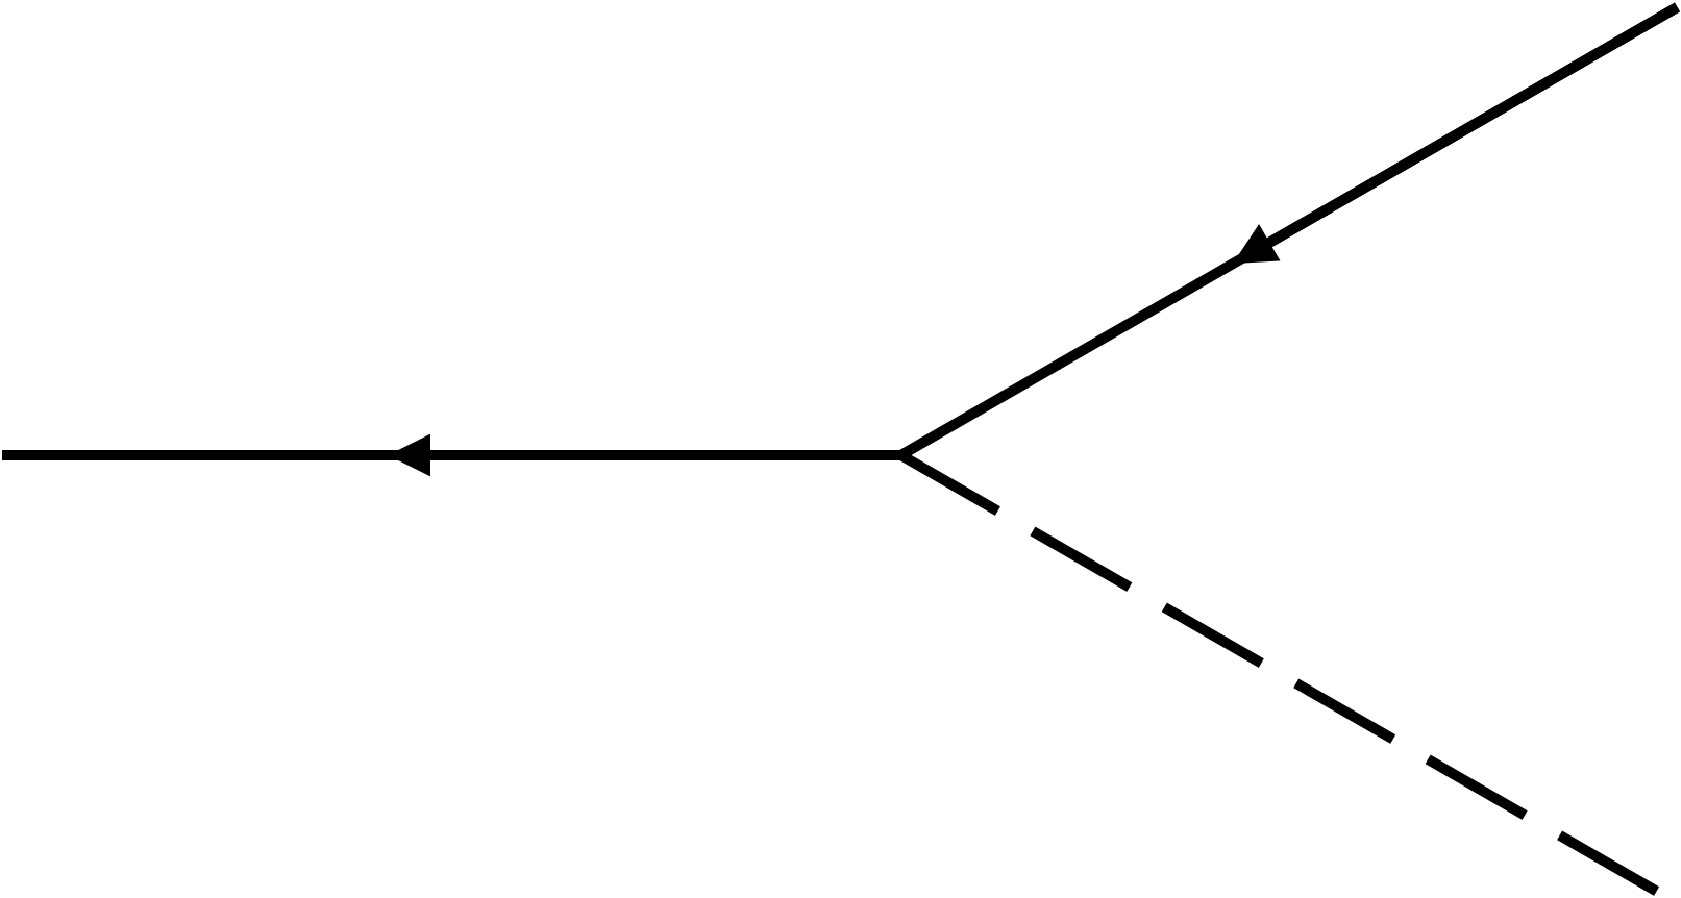
\includegraphics[width = 0.5\textwidth, height = 0.25\textwidth]{figures/interaction.pdf}
    \caption{Interaction}
\end{figure}


\subsection{Order-by-order Solution to RGPEP Equation}
\subsubsection{$\mathcal{O}(g)$ Solution}
\label{sec:first-order}
At first order in $g$, the RGPEP equation is 

\begin{equation}
    \label{eq:first-order}
    \frac{dH^{(1)}(t)}{dt} = \left[\left[H_0, H^{(1)}(t) \right], H_0 \right].
\end{equation}

We can see that the inner commutator in equation \ref{eq:first-order} is the same form as the generator, but at first order. 
Thus, we define $\mathcal{G}^{(1)}(t) = \left[H_0,  H^{(1)}(t)\right]$.
The first step in solving equation \ref{eq:first-order}, is by working out this commutator. 
This will also elucidate some structure of this method that will greatly simplify calculations.

The free Hamiltonian term, written in terms of ladder operators given in equations \ref{eq:phi}, \ref{eq:psi} is 

\begin{equation}
    \label{eq:H-free-ladder}
    H_0 = \int_q \frac{m^2}{q^+}\left(b_q^\dagger b_q + d_q^\dagger d_q \right) + \int_q \frac{\mu^2}{q^+}a_q^\dagger a_q,
\end{equation}

where $$\int_q \equiv \int \frac{dq^+}{4\pi}.$$

While too long to write out $H_Y$ in this form, looking at one term in the expansion of $\bar \psi \psi \phi$ in equation \ref{eq:H-3}, and working out its commutator with equation \ref{eq:H-free-ladder} will give the general form of the generator.

One term in \ref{eq:H-3} is $$\int_{q_1 q_2 q_3}C_{q_1, q_2, q_3}(t)\theta(-q_1^+)\theta(q_2^+)\theta(q_3^+) \bar u(-q_1) u(q_2) b_{-q_1}^\dagger b_{q_2} a_{q_3}.$$
The commutator that must be worked out to obtain the corresponding term of $\mathcal{G}^{(1)}(t)$ is

$$
    \left[\int_q \frac{m^2}{q^+}\left(b_q^\dagger b_q + d_q^\dagger d_q \right) + \int_q \frac{\mu^2}{q^+}a_q^\dagger a_q,  \int_{q_1 q_2 q_3}C_{q_1, q_2, q_3}(t)\theta(-q_1^+)\theta(q_2^+)\theta(q_3^+) \bar u(-q_1) u(q_2) b_{-q_1}^\dagger b_{q_2} a_{q_3}\right].
$$

This commutator equals $$\int_{q_1 q_2 q_3}-\left(q_1^- + q_2^- + q_3^- \right)C_{q_1, q_2, q_3}(t)\theta(-q_1^+)\theta(q_2^+)\theta(q_3^+) \bar u(-q_1) u(q_2) b_{-q_1}^\dagger b_{q_2} a_{q_3}.$$
This is simply the original term from $H^{(1)}(t)$ in the commutator, modified by $-\left(q_1^- + q_2^- + q_3^- \right)$, the negative sum of the total momentum flowing into the vertex. 
It turns out that working out the commutator between $H_0$ and every term in $H^{(1)}(t)$ yields this same form.
Thus, the generator, at first order, is simply a modification of the first order Hamiltonian modified by the negative sum of momentum flowing into each vertex:

\begin{equation}
    \mathcal{G}^{(1)}(t) = -\mathcal{Q}^- H^{(1)}(t).
\end{equation}

Now that $\mathcal{G}^{(1)}(t)$ has been worked out, the full right-hand side of equation \ref{eq:first-order} can be determined:

\begin{align*}
    \left[\mathcal{G}^{(1)}(t), H_0 \right] &= \left[-\mathcal{Q}^- H^{(1)}(t), H_0 \right]\\
    &= -\mathcal{Q}^-\left[H^{(1)}(t), H_0 \right]\\
    &= -\mathcal{Q}^- \left(-\mathcal{G}^{(1)}(t) \right)\\
    &= -\left(\mathcal{Q}^-\right)^2H^{(1)}(t).
\end{align*}

Thus, equation \ref{eq:first-order}, in terms of the parameterized coefficient, which then defines $H^{(1)}(t)$ is:

\begin{equation*}
    \frac{dC_{q_1, q_2, q_3}(t)}{dt} = -(q_1^- + q_2^- + q_3^-)^2C_{q_1, q_2, q_3}(t),
\end{equation*}

whose solution, in terms of the Hamiltonian gives:

\begin{equation}
    H^{(1)}(t) = 4\pi g\int_{q_1 q_2 q_3}\delta(q_1^+ + q_2^+ +q_3^+)e^{-t\left(q_1^- + q_2^- + q_3^-\right)^2}:\bar \psi(-q_1) \psi(q_2) \phi(q_3):.
\end{equation}

The exponential term is referred to as a \textit{form factor}, which regulates the 3-point interaction vertices by exponentially damping terms whose energy going into a vertex is large.

% The first order part of $H$ is given in equation \ref{eq:yukawa-hamiltonian}.
% To determine how $H^{(1)}$ evolves in $t$, we must add explicit \textit{t}-dependence to the coefficients of $H^{(1)}$.
% This is done by substituting the coefficients in front of each product of creation and annihilation operators with arbitrary coefficients that depend not only on momenta, but also $t$. 
% For example, the coefficient in front of $b_i^\dagger b_j a_k$ changes from $$4\pi \delta\left(p_i^+ - p_j^+ - p_k^+ \right)\bar u(p_i) u(p_j) \rightarrow c_{ijk}(t)$$  
% The rest of the coefficients can similarly be exchanged for a paramterized version, where it is important to modify the coefficient in a way that it is clear which term it modifies:

% \begin{align}\nonumber
%     4\pi \delta\left(p_i^+ + p_k^+ - p_j^+ \right)\bar{u}(p_i) u(p_j) &\rightarrow c^*_{ikj}(t)\\ \nonumber
%     4\pi \delta\left(p_i^+ - p_j^+ - p_k^+ \right)\bar{v}(p_j) v(p_i) &\rightarrow \bar{c}_{ijk}(t) \\ \nonumber
%     4\pi \delta\left(p_i^+ + p_k^+ - p_j^+ \right)\bar{v}(p_j) v(p_i) &\rightarrow \bar c^*_{ikj}(t)\\ \nonumber
%     4\pi \delta\left(p_i^+ + p_j^+ - p_k^+ \right)\bar{u}(p_i) v(p_j) &\rightarrow \tilde c_{ijk}(t)\\ \nonumber
%     4\pi \delta\left( p_k^+ - p_i^+ - p_j^+ \right)\bar{v}(p_j) u(p_i) &\rightarrow \tilde c^*_{kij}(t)\\ \nonumber
% \end{align}

% The Hamiltonian now assumes a simpler form:

% \begin{align}
%     \label{eq:H-first-order-c-coeffs}
%     H^{(1)}(t) = g\int_i \int_j \int_k &\left(c_{ijk}(t)b_i^\dagger b_j a_k + c_{ikj}^*(t) b_i^\dagger b_j a_k^\dagger + \bar c_{ijk}(t) d_i^\dagger d_j a_k \right. \\ \nonumber
%     & \left. \bar c^*_{ikj}(t) d^\dagger_i d_j a_k^\dagger + \tilde c_{ijk}(t)b_i^\dagger d_j^\dagger a_k + \tilde c^*_{kij}(t) b_i d_j a_k^\dagger \right).
% \end{align}

% where
% \begin{equation}
%     \int_i \rightarrow \int_0^\infty \frac{dp_i^\dagger}{4\pi p_i^+}
% \end{equation}

% We similarly modify the free part of the Hamiltonian as

% \begin{equation}
%     H_0 = \int_n B_n b_n^\dagger b_n + \int_n D_n d_n^\dagger d_n + \int_n A_n a_n^\dagger a_n.
% \end{equation}

% The inner commutator in equation \ref{eq:first-order} modifies each term in the Hamiltonian by the coefficients in the free part $H_0$.
% For example, the first term in equation \ref{eq:H-first-order-c-coeffs} corresponds to fermion $+$ boson in, fermion out. 
% The term thus gets modified by $\left(B_i - D_j - A_k\right)$.
% Continuing this with every term arrives at:

% \begin{align}
%     \label{eq:first-order-inner-commutator}
%     \left[H_0, H^{(1)}(t) \right] &= g\int_i \int_j \int_k \left(\left(B_i - B_j - A_k \right)c_{ijk}(t)b_i^\dagger b_j a_k + \left(B_i + A_k - B_j\right)c_{ikj}^*(t) b_i^\dagger b_j a_k^\dagger + \left(D_i - D_j - A_k \right)\bar c_{ijk}(t) d_i^\dagger d_j a_k \right. \\ \nonumber
%     & \left. \left(D_i + A_k - D_j\right)\bar c^*_{ikj}(t) d^\dagger_i d_j a_k^\dagger + \left(B_i + D_j - A_k\right)\tilde c_{ijk}(t)b_i^\dagger d_j^\dagger a_k + \left(A_k - B_i - D_j \right)\tilde c^*_{kij}(t) b_i d_j a_k^\dagger \right).
% \end{align}

% To get the full right hand side of equation \ref{eq:first-order}, we do another commutator of equation \ref{eq:first-order-inner-commutator} with $H_0$, which gives another factor of the modificiations of the form $B_i + D_j - A_k$, with a negative sign ($H_0$ is on the right of the commutator now). 

% \begin{align}
%     \label{eq:RHS-first-order}
%     \left[\left[H_0, H^{(1)}(t) \right], H_0\right] = g\int_i \int_j \int_k &\left(-\left(B_i - B_j - A_k \right)^2c_{ijk}(t)b_i^\dagger b_j a_k - \left(B_i + A_k - B_j\right)^2c_{ikj}^*(t) b_i^\dagger b_j a_k^\dagger \right. \\ \nonumber
%     &\left. - \left(D_i - D_j - A_k \right)^2\bar c_{ijk}(t) d_i^\dagger d_j a_k -\left(D_i + A_k - D_j\right)^2\bar c^*_{ikj}(t) d^\dagger_i d_j a_k^\dagger\right. \\ \nonumber
%     & \left.  - \left(B_i + D_j - A_k\right)^2\tilde c_{ijk}(t)b_i^\dagger d_j^\dagger a_k - \left(A_k - B_i - D_j \right)^2\tilde c^*_{kij}(t) b_i d_j a_k^\dagger \right).
% \end{align}

% If we differentiate equation \ref{eq:H-first-order-c-coeffs}, the coefficients in $t$ now become derivatives in $t$.
% Term by term, we can equate the derivatives on the left hand side of \ref{eq:first-order} with the corresponding term from equation \ref{eq:RHS-first-order}.
% For example, 

% \begin{equation}
%     \frac{d}{dt}c_{ijk}(t) = -\left(B_i - B_j - A_k \right)^2 c_{ijk}(t)
% \end{equation}

% which has solution 

% \begin{equation}
%     c_{ijk}(t) = c_{ijk}(0)e^{-\left(B_i - B_j - A_k \right)^2t}
% \end{equation}
% where $c_{ijk}(0)$ comes from the initial Hamiltonian we wrote down: $c_{ijk}(0) = 4\pi \delta\left(p_i^+ - p_j^+ - p_k^+ \right)\bar u(p_i) u(p_j)$.
% Thus, the full first order solution is given as:
 
% \begin{align}
%     &H^{(1)}(t) = \int_0^\infty\int_0^\infty\int_0^\infty \frac{dp_i^+dp_j^+dp_k^+}{\left(4\pi \right)^3 p_i^+ p_j^+ p_k^+}\left(4\pi \delta\left(p_i^+ - p_j^+ - p_k^+ \right) \bar u(p_i) u(p_j) e^{-\left(\frac{m_F^2}{p_i^+} - \frac{m_F^2}{p_j^+} - \frac{m_B^2}{p_k^+} \right)^2t} b_i^\dagger b_j a_k \right.\\ \nonumber
%     &\left. +4\pi \delta\left(p_i^+ + p_k^+- p_j^+  \right) \bar u(p_i) u(p_j) e^{-\left(\frac{m_F^2}{p_i^+} + \frac{m_B^2}{p_k^+} - \frac{m_F^2}{p_j^+}  \right)^2t} b_i^\dagger b_j a_k^\dagger + 4\pi \delta\left(p_i^+ - p_j^+ - p_k^+ \right) \bar v(p_j) v(p_i) e^{-\left(\frac{m_{\bar F}^2}{p_i^+} - \frac{m_{\bar F}^2}{p_j^+} - \frac{m_B^2}{p_k^+} \right)^2t} d_i^\dagger d_j a_k \right. \\ \nonumber
%     &\left.  +4\pi \delta\left(p_i^+ + p_k^+ - p_j^+ \right) \bar v(p_j) v(p_i) e^{-\left(\frac{m_{\bar F}^2}{p_i^+} + \frac{m_B^2}{p_k^+} - \frac{m_{\bar F}^2}{p_j^+}  \right)^2t} d_i^\dagger d_j a_k^\dagger + 4\pi \delta\left(p_i^+ + p_j^+ - p_k^+ \right) \bar u(p_i) v(p_j) e^{-\left(\frac{m_F^2}{p_i^+} + \frac{m_{\bar F}^2}{p_j^+} - \frac{m_B^2}{p_k^+} \right)^2t} b_i^\dagger d_j^\dagger a_k \right. \\ \nonumber
%     & \left.  +4\pi \delta\left(p_i^+ + p_j^+ - p_k^+ \right) \bar v(p_j) u(p_i) e^{-\left(\frac{m_B^2}{p_k^+} - \frac{m_F^2}{p_i^+} - \frac{m_{\bar F}^2}{p_j^+}  \right)^2t}b_i d_j a_k^\dagger\right)\\ \nonumber
% \end{align}

% It is important to note that the exponentials in $t$ are referred to as \textit{form factors}.

% \subsubsection{$\mathcal{O}(g^2)$ Solution}
% \label{sec:second-order}
% At second order in $g$, the RGPEP equation is more involved:

% \begin{equation}
%     \label{eq:rgpep-second-order}
% g^2\dot{H}^{(2)}(t) = \left[\left[H_0, g^2H^{(2)}(t)\right], H_0\right] + \left[\left[H_0, gH^{(1)}(t)\right],gH^{(1)}(t)\right]
% \end{equation}

% At first glance at equation \ref{eq:yukawa-hamiltonian}, it appears as if only the instantaneous terms make up $H^{(2)}(t)$. 
% However, it is important to add to $H^{(2)}(t)$ higher order terms arising from combining two $\mathcal{O}(g)$ interactions. 
% Computing the second commutator in equation \ref{eq:rgpep-second-order} reveals the $\mathcal{O}(g^2)$ interaction terms. 
% This commutator is written as $$\left[\mathcal{G}^{(1)}(t), H^{(1)}(t) \right].$$
% Using Wick's theorem, we can simplify this commutator \footnote{For example, to compute $\left[b_n^\dagger b_n, b_x^\dagger b_y a_z \right] = b_n^\dagger b_nb_x^\dagger b_y a_z - b_x^\dagger b_y a_zb_n^\dagger b_n$, we first normal order both terms and induce Dirac deltas: $b_n^\dagger b_nb_x^\dagger b_y a_z - b_x^\dagger b_y a_zb_n^\dagger b_n = b_n^\dagger \left(\delta_{nx} - b_x^\dagger b_n \right)b_y a_z - b_x^\dagger \left(\delta_{ny} - b_n^\dagger b_y \right)b_n a_z = \delta_{nx}b_n^\dagger b_y a_z - \delta_{ny}b_x^\dagger b_n a_z$. This is the difference between normal ordered contractions in the last line of equation \ref{eq:commutator-to-contractions}}: 

% \begin{align}
%     \label{eq:commutator-to-contractions}
%     \left[\mathcal{G}^{(1)}(t), H^{(1)}(t) \right] &= \mathcal{G}^{(1)}(t)H^{(1)}(t) - H^{(1)}(t)\mathcal{G}^{(1)}(t)\\ \nonumber
%     &= :\mathcal{G}^{(1)}(t)H^{(1)}(t): + :C\left(\mathcal{G}^{(1)}(t)H^{(1)}(t)\right): - :H^{(1)}(t)\mathcal{G}^{(1)}(t): - :C\left(H^{(1)}(t)\mathcal{G}^{(1)}(t) \right):\\ \nonumber
%     &=:C\left(\mathcal{G}^{(1)}(t)H^{(1)}(t)\right): - :C\left(H^{(1)}(t) \mathcal{G}^{(1)}(t)\right):.\\ \nonumber
% \end{align} 

% Here, it is assumed that $:\mathcal{G}^{(1)}(t)H^{(1)}(t): = H^{(1)}(t)\mathcal{G}^{(1)}(t): $ since the number of fermions (antifermions) always come in pairs in any quantum field theory.

% We can continue simplifying equation \ref{eq:commutator-to-contractions}:

% \begin{align}
%     \label{eq:full-simplification-of-GH-comm}
%     \left[\mathcal{G}^{(1)}(t), H^{(1)}(t) \right] &= :C\left(\mathcal{G}^{(1)}(t)H^{(1)}(t)\right): - :C\left(H^{(1)}(t) \mathcal{G}^{(1)}(t)\right):\\ \nonumber
%     &= \sum_{D_1, D_2} \left(:C\left(\mathcal{G}_{D_1}^{(1)}(t)H_{D_2}^{(1)}(t)\right): - :C\left(H^{(1)}_{D_1}(t) \mathcal{G}^{(1)}_{D_2}(t)\right) \right) \\ \nonumber
%     &= \sum_{contractions} \left(\mathcal{P}_A + \mathcal{P}_B -2\mathcal{P}_C  \right)V_1(0) V_2(0)T_{contraction}
% \end{align}

% To understand the final form of equation \ref{eq:full-simplification-of-GH-comm}, we note $D_i \in \{\text{Yukawa interactions} \}$. 
% Thus, we calculate contractions of every pair of interaction terms in $H^{(1)}(t)$ (since interaction terms in $\mathcal{G}^{(1)}(t)$ are the same, up to some coefficient modifications).
% After writing down every possible contraction, we now have $\mathcal{O}(g^2)$ interaction diagrams, labeled by $T_{contraction}$, which describes the ladder operator structure of the term. 
% Instead of meticulously keeping track of indices, the last line in equation \ref{eq:full-simplification-of-GH-comm} allows you to take a given contraction from two interactions, and gives the modification to the coefficient needed to write out the commutator in equation \ref{eq:full-simplification-of-GH-comm}.
% An example is given in figures \ref{fig:D1D2} and \ref{fig:contraction}.

% % \begin{figure}
% %     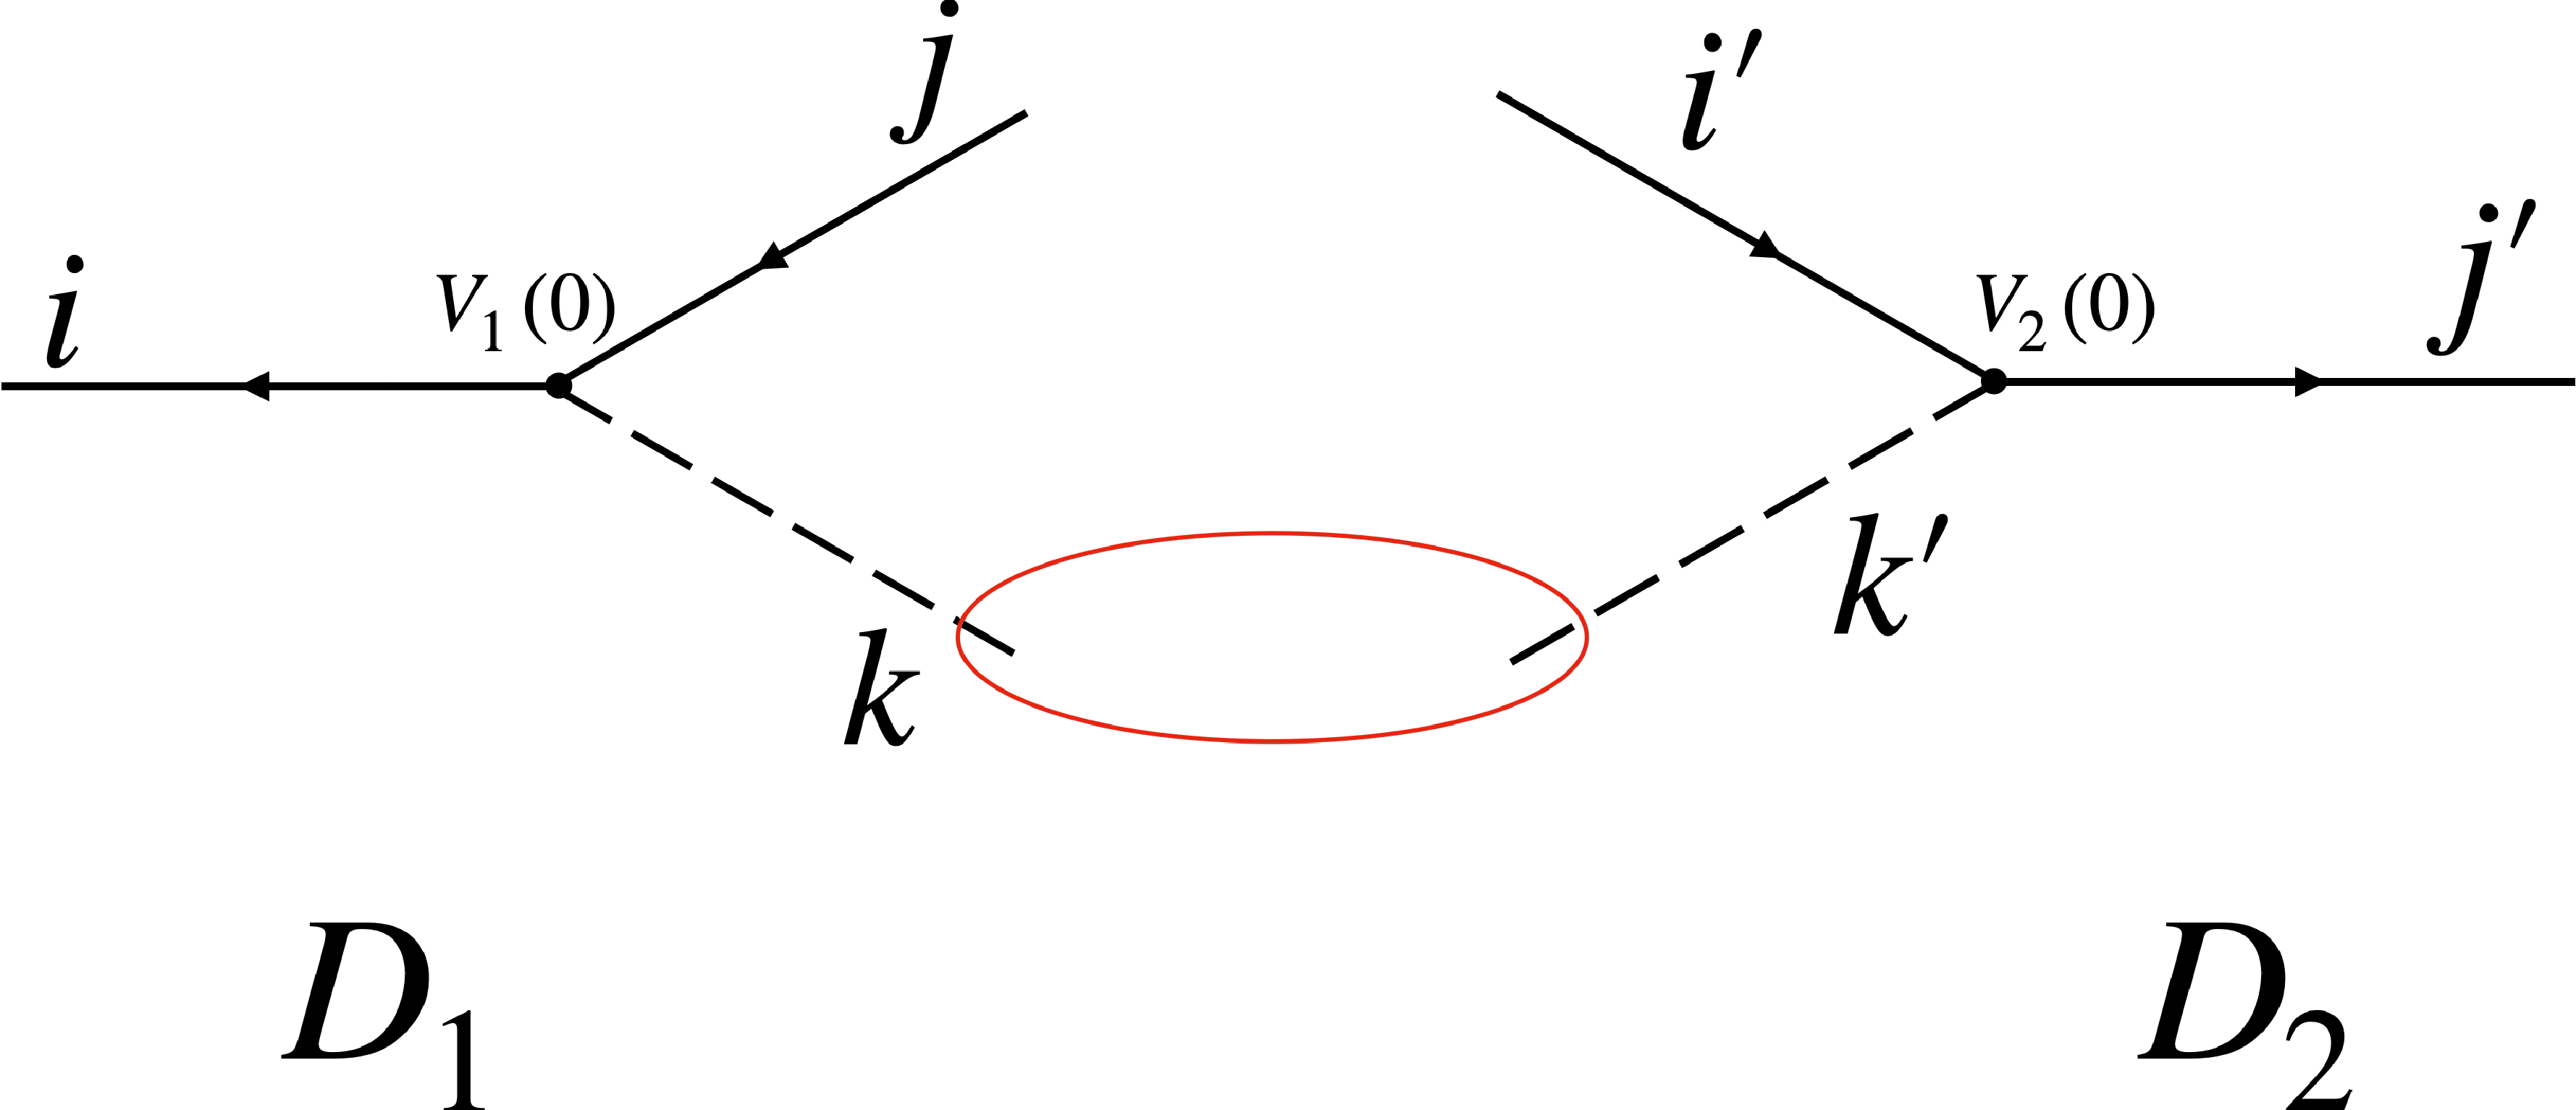
\includegraphics[width = 0.75\textwidth]{figures/D1D2.pdf}
% %     \caption{Two interaction diagrams, $D1$ and $D2$ are chosen. There is only one possible contraction, which is circled in red.}
% %     \label{fig:D1D2}
% % \end{figure}

% % \begin{figure}
% %     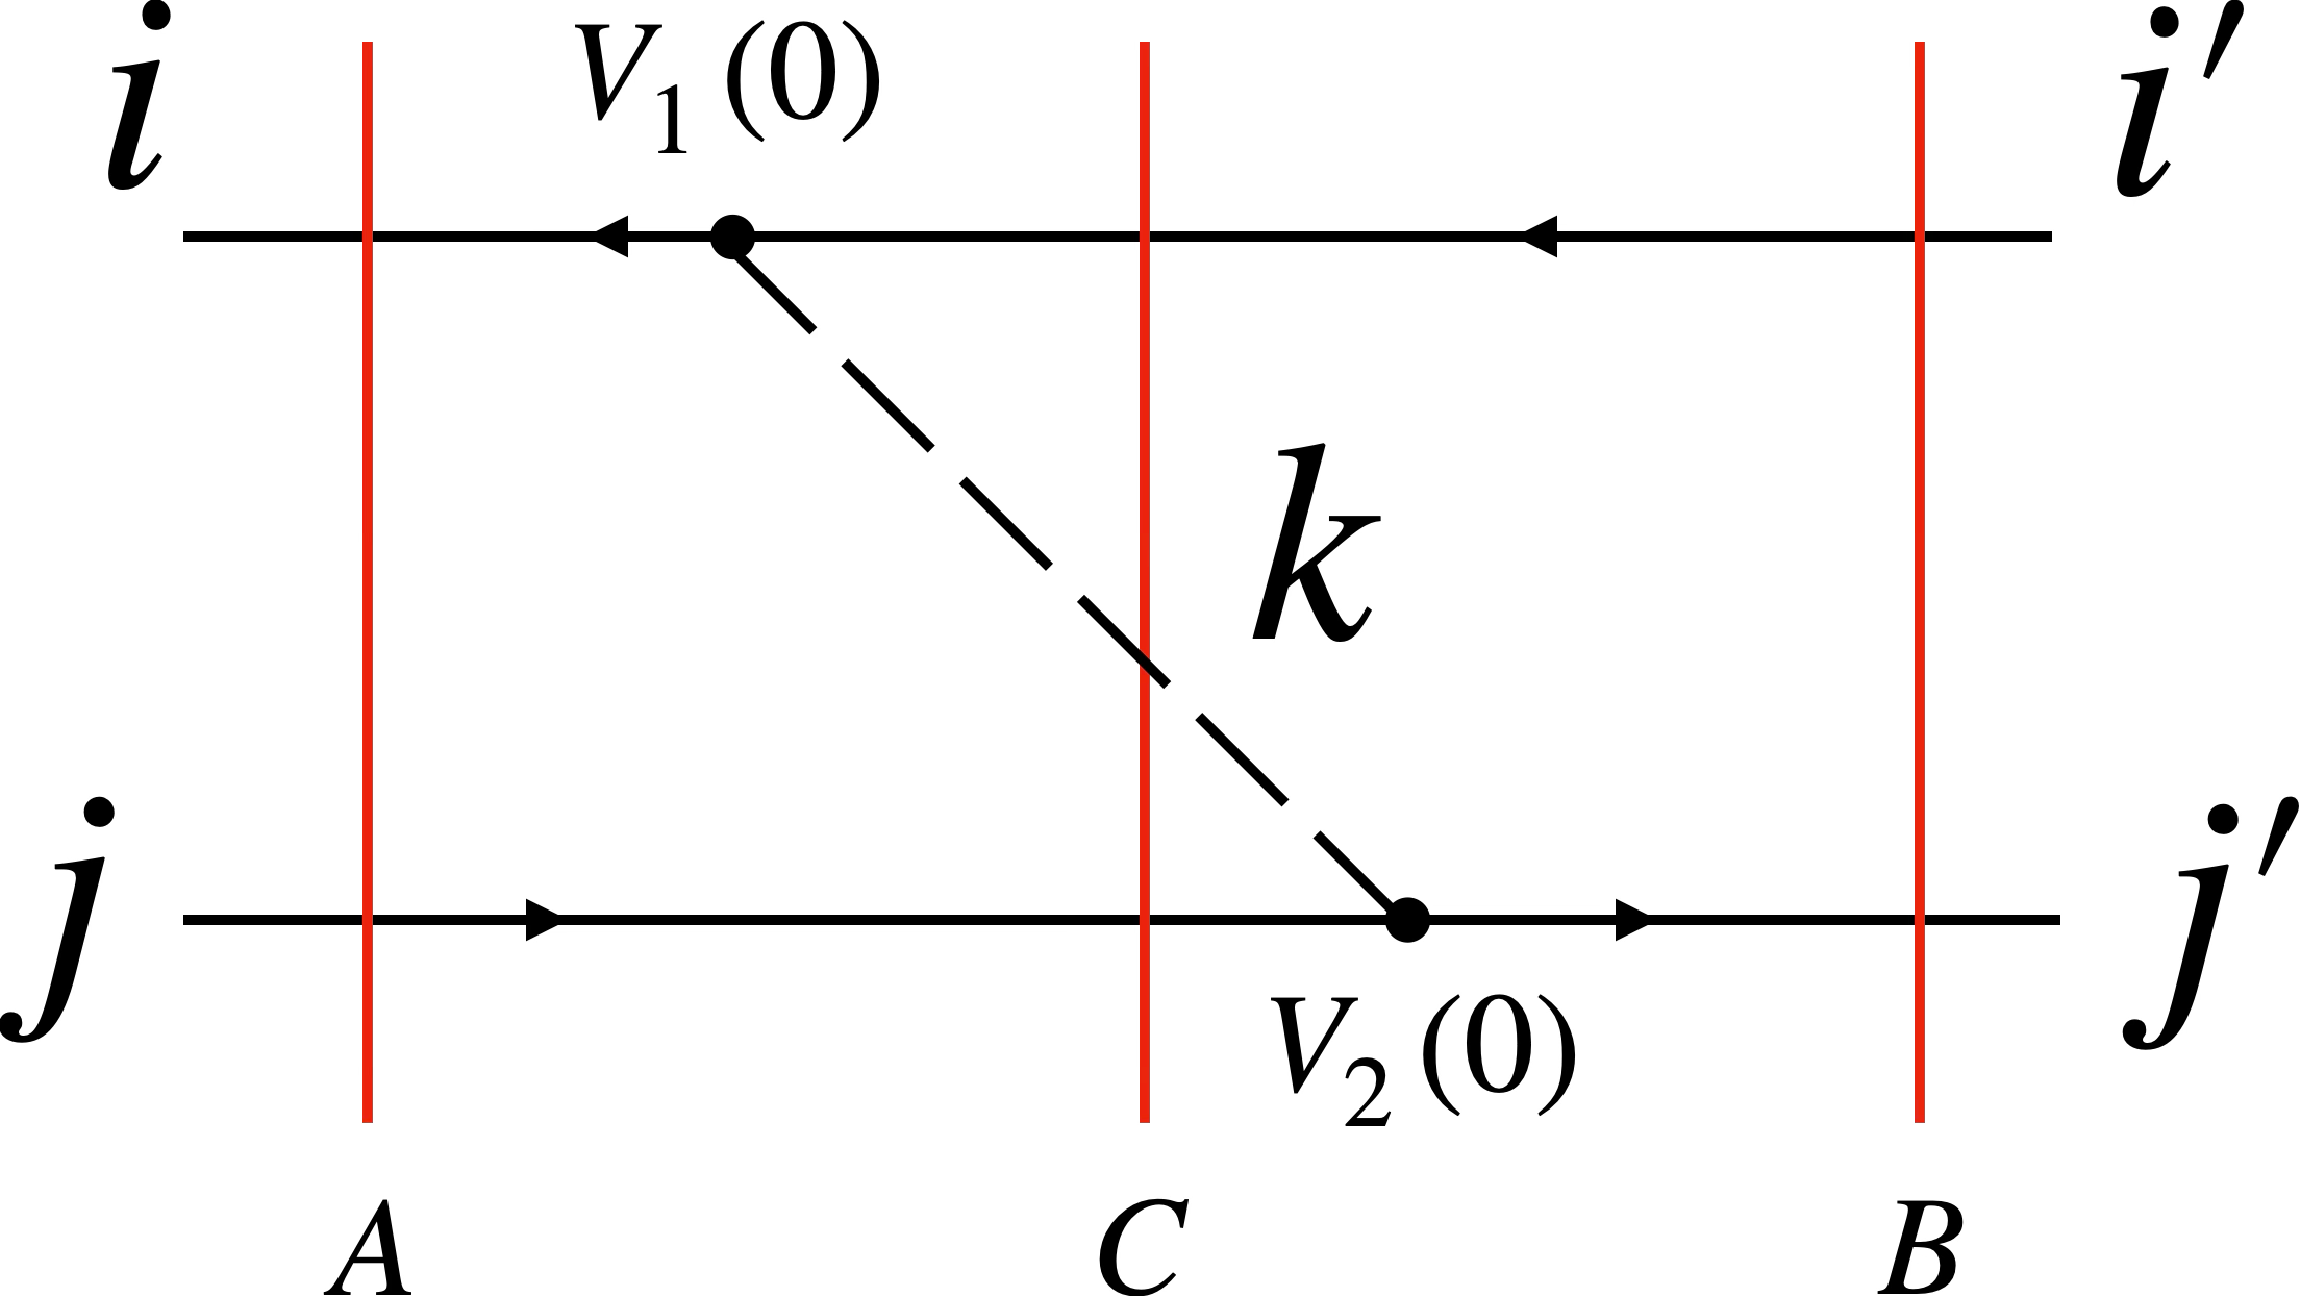
\includegraphics[width = 0.6\textwidth]{figures/contraction.pdf}
% %     \caption{When we contract the bosons in $D1$ and $D2$ in figure \ref{fig:D1D2}, we get an $\mathcal{O}(g^2)$ diagram. Keeping track of the original indices is unnecesssary, if you label them in a consistent way.}
% %     \label{fig:contraction}
% % \end{figure}

% For this example, $\mathcal{P}_A + \mathcal{P}_B - 2\mathcal{P}_2 = c_i - c_{i'} + c_j - c_{j'} - 2c_k$ (i.e. $\mathcal{P}_i$ is the sum of momentum along the red line of $i$), and $V_1(t) = c_{ijk}(t), V_2(t) = \bar c^*_{ijk}(t)$. Thus, $$\left[\mathcal{G}^{(1)}(t), H^{(1)}(t) \right]_{D_1, D_2} = \int_{ijki'j'}\left(c_i - c_{i'} + c_j - c_{j'} - 2c_k \right)c_{ijk}(0)\bar c^*_{ijk}(0) b_i^\dagger b_{i'}d_j^\dagger d_{j'}.$$

% Doing this $\forall D_1, D_2 \in \{interactions\}$, we obtain $\left[\mathcal{G}^{(1)}(t), H^{(1)}(t) \right]$. 
% The important information obtained from computing all of the contractions is that you can now write down a parameterized form for $\mathcal{O}(g^2)$ terms to add to $H^{(2)}(t)$. 
% Again, using the example of figures \ref{fig:D1D2} and \ref{fig:contraction}, we could parameterize this addition to $H^{(2)}(t)$ as $$H^{(2)}_{D_1, D_2}(t) = \int_{ijki'j'}K(t)  b_i^\dagger b_{i'}d_j^\dagger d_{j'},$$ where $K(t)$ is a parameterized coefficient to be determined by solving equation \ref{eq:rgpep-second-order}. \gus{Change $D1, D2$ subscript in above equation to be a figure of the corresponding diagram}.

% Now that we have a parameterized form of $H^{(2)}(t)$, complete with additional terms from the contractions, we can calculate the first commutator in equation \ref{eq:rgpep-second-order}.

% For a given term in $H^{(2)}(t)$, the commutator $\left[\left[H_0, g^2H^{(2)}(t)\right], H_0\right]$ is simple to calculate. 
% In a similar way that $\left[\left[H_0, gH^{(1)}(t)\right], H_0\right]$ was calculated, this second order commutator will modify the given term by $-\left(\mathcal{P}_A - \mathcal{P}_B\right)^2$ (refer to figure \ref{fig:contraction}).

% We can finally write down the general form of the differential equation that comes from equation \ref{eq:rgpep-second-order} for a given second order diagram $D$ with parameterized coefficient in $H^{(2)}(t)$, $K(t)$:

% \begin{equation}
%     \label{eq:second-order-DE}
%     \frac{d}{dt}K_D(t) = -\left(\mathcal{P}_A - \mathcal{P}_B \right)^2 K_D(t) + \left(\mathcal{P}_A + \mathcal{P}_B - 2\mathcal{P}_C \right)V_1(0)e^{-p_{V_1}^2t}V_2(0)e^{-p_{V_2}^2t}
% \end{equation}

% where $p_{V_i}^2$ is sum of $c_j's$ into $V_i$ minus sum of $c_j's$ out of $V_i$. 
% For the example of $D_1$ in figure \ref{fig:D1D2}, $p_{V_1} = \left(c_i - c_j - c_k \right)$.

% The general solution to equation \ref{eq:second-order-DE} is \footnote{A differential equation of the form $\frac{dy}{dt} = -p(t)y(t) + q(t)$ has the general solution $y(t) = e^{-h(t)}\int e^{h(t)}q(t) + Ce^{-h(t)}$, where $h(t) = \int dt p(t)$}:

% \begin{equation}
%     K_D(t) = \frac{\left(\mathcal{P}_A + \mathcal{P}_B - 2\mathcal{P}_C \right)V_1(0)V_2(0)}{p_{V_1}^2 + p_{V_2}^2 - \left(\mathcal{P}_A - \mathcal{P}_B \right)^2} \left(e^{-\left( \mathcal{P}_A - \mathcal{P}_B\right)^2t} - e^{-\left(p_{V_1}^2 + p_{V_2}^2\right)t} \right) + K_D(0)
% \end{equation}

% The last thing to note before writing out the solution to \ref{eq:rgpep-second-order} is that we must take into account the original instantaneous second order diagrams present in \ref{eq:yukawa-hamiltonian}. 
% The first commutator in \ref{eq:rgpep-second-order} will be non-zero for this interaction, and can simply be wrote down as the original term, modified by $-\left(\mathcal{P}_A - \mathcal{P}_B \right)^2$. 
% Each second order term in the Hamiltonian is now written out explicitly in table \ref{tab:H2}:


\subsubsection{$\mathcal{O}(g^2)$ Solution}
\label{sec:second-order}

At second order in $g$, the RGPEP equation is

\begin{equation}
    \label{eq:second-order}
    \frac{dH^{(2)}(t)}{dt} = \left[\left[H_0, H^{(2)}(t)\right], H_0\right] + \left[\left[H_0, H^{(1)}(t)\right],H^{(1)}(t)\right].
\end{equation}
This equation is more involved than the first order equation; however, looking at the parts of the sum on the right-hand side individually is insightful.

First, look at $\left[\mathcal{G}^{(1)}(t),H^{(1)}(t)\right],$ where the substitution $\mathcal{G}^{(1)}(t) = \left[H_0, H^{(1)}(t)\right]$ was made.

\begin{align*}
    \left[\mathcal{G}^{(1)}(t),H^{(1)}(t)\right] &= \left(-\mathcal{Q}^- H^{(1)}(t)\right)H^{(1)}(t) - H^{(1)}(t)\left(-\mathcal{Q}^- H^{(1)}(t)\right)\\
    &= :\left(-\mathcal{Q}^- H^{(1)}(t)\right)H^{(1)}(t): + :C\left[\left(-\mathcal{Q}^- H^{(1)}(t)\right)H^{(1)}(t)\right]:\\
    & - :H^{(1)}(t)\left(-\mathcal{Q}^- H^{(1)}(t)\right): - :C\left[H^{(1)}(t)\left(-\mathcal{Q}^- H^{(1)}(t)\right)\right]:\\
    &= :C\left[\left(-\mathcal{Q}^- H^{(1)}(t)\right)H^{(1)}(t)\right]: - :C\left[H^{(1)}(t)\left(-\mathcal{Q}^- H^{(1)}(t)\right)\right]:.
\end{align*}

The last line of this equality is true because there are an equal number of fermions and antifermions, thus their normal orderings cancel.
This difference in contractions can be simplified to the following expression:

\begin{equation}
    \label{eq:GH-comm}
    \left[\mathcal{G}^{(1)}(t),H^{(1)}(t)\right] = \int\limits_{\substack{q_1, q_2, q_3 \\ q_1', q_2', q_3'}} \delta \left(q_1^+ + q_2^+ + q_3^+ \right)\delta \left(q_1'^+ + q_2'^+ + q_3'^+ \right)A(t):C\left[H^{(1)}(t)H^{'(1)}(t) \right]:
\end{equation}
where $$A(t) = \left[-\left(q_1^+ + q_2^+ + q_3^+ \right) + \left(q_1'^+ + q_2'^+ + q_3'^+ \right)\right]f(t) f'(t).$$
A pictorial proof of equation \ref{eq:GH-comm} will be given in the appendix.

To determine the first commutator in equation \ref{eq:second-order}, $H^{(2)}(t)$ must be parameterized similar to the $\mathcal{O}(g)$ solution. 
$H^{(2)}(t)$ will not only contain the $\mathcal{O}(g^2)$ instantaneous terms that exist in the canonical Hamiltonian even when $t = 0$, but will also include second order terms that arise from the contraction of two first order interaction vertices. 
Thus, the parameterization is

\begin{align}
    H^{(2)}(t) &= 2\pi g^2 \int\limits_{\substack{q_1, q_2\\ q_3, q_4}} \delta \left(q_1^+ + q_2^+ + q_3^+ + q_4^+ \right) B(t):\bar \psi(-q_1) \phi(q_2)\frac{\gamma^+}{q_3^+ + q_4^+} \phi(q_3) \psi(q_4): \\ \nonumber
    &+ g^2 \int\limits_{\substack{q_1, q_2, q_3\\ q_1', q_2', q_3'}} \delta \left(q_1^+ + q_2^+ + q_3^+ \right) \delta \left(q_1'^+ + q_2'^+ + q_3'^+ \right)B(t):C\left[\bar \psi(-q_1)\psi(q_2)\phi(q_3)\bar \psi(-q_1')\psi(q_2')\phi(q_3') \right]:.
\end{align}

Each second order interaction term has its own solution to equation \ref{eq:second-order}. 
The easiest interaction terms to solve are the instantaneous interaction terms. 
These can be solved in the same way the first order terms are solved, that is they pick up a form factor:

$$
H^{(2)}_{\text{inst.}}(t) = 2\pi g^2 \int\limits_{\substack{q_1, q_2\\ q_3, q_4}} \delta \left(q_1^+ + q_2^+ + q_3^+ + q_4^+ \right) e^{-t \left(q_1^+ + q_2^+ + q_3^+ + q_4^+ \right)^2}:\bar \psi(-q_1) \phi(q_2)\frac{\gamma^+}{q_3^+ + q_4^+} \phi(q_3) \psi(q_4):.
$$

The commutator between contracted $\mathcal{O}(g^2)$ terms in $H^{(2)}(t)$ and $H_0$ in equation \ref{eq:second-order} isn't as simple as the instantaneous terms, which follow the same procedure as section \ref{sec:first-order} (i.e. picking up a factor of $-\mathcal{Q}$, the sum of $q_i$'s into the vertices).

$\frac{dy}{dt} = -p(t)y(t) + q(t)$ has the general solution $y(t) = e^{-h(t)}\int e^{h(t)}q(t) + Ce^{-h(t)}$, where $h(t) = \int dt p(t)$

%\bibliography{refs/citations}

\appendix

\section{Momentum Space Representation of the Yukawa Hamiltonian}
\label{sec:hamiltonian}

In position space, the Hamiltonian density is 

\begin{align}
    H_0 &= \frac{m^2}{2}
\end{align}
\section{Discretized Lightcone Quantization (DLCQ)}
\label{sec:dlcq}

One can discretize equation \ref{eq:yukawa-hamiltonian} directly by discretizing each piece individually. 
Alternatively, and perhaps more straightforward, one may discretize the fields before writing out the Hamiltonian.
Also, since we want the Hamiltonian in momentum space, we perform a Fourier transformation of the discretized fields. 

The fields are discretized in a 1+1D box of length $x^- \in \{-L, L\}$ which, due to boundary conditions and symmetry requirements for fermions and bosons, leads to discretized momenta, $p_k$ given as 

$$p_k = \frac{2\pi k}{L}; k = 
\begin{cases}
    \frac{1}{2},\frac{3}{2},\frac{5}{2} \dots ; \text{fermions}\\
    1, 2, 3, \dots ; \text{bosons}
\end{cases}$$

For the scalar field, $\phi(x)$, $$\phi(x) = \sum_{k = 1}^\infty \frac{1}{\sqrt{4\pi k}}\left(a_{i_k} e^{-ip_k x} + a_{i_k}^\dagger e^{ip_k x} \right).$$
Here, the subscript $i_k$ refers to a particular index corresponding to mode $k$. 
We can transpose $\phi(x)$ to its corresponding momentum space field, denoted by $\tilde \phi(k)$: $$\tilde \phi(k) = \int_{-L}^L dx^- e^{\frac{i}{2}q_k^+ x^-}\phi(x).$$
The exponent in the exponential in this equation comes from the dot product in lightfront coordinates and asserting a fixed $x^+ = 0$ plane. 
Plugging in the form of $\phi(x)$, we obtain the discretized scalar field in momentum space as:

\begin{equation}
    \tilde \phi(k) = 2L \frac{\theta(k)a_{i_k} + \theta(-k)a_{-i_k}}{\sqrt{4\pi |k|}}.
\end{equation}

The fermionic field is $$\psi(x) = \sum_{k = 1/2}^\infty \frac{1}{\sqrt{4\pi k}}\left(b_{i_k}u(p_k) e^{-ip_k x} + v(p_k)d_{i_k}^\dagger e^{ip_k x} \right)$$ where $$u(p_k) = \frac{1}{\sqrt{p_k^+}}\left[\begin{matrix} p^+_k \\ m \end{matrix}\right],$$ $$v(p_k) = \frac{1}{\sqrt{p_k^+}}\left[\begin{matrix} -p^+_k \\ m \end{matrix}\right].$$
After the same Fourier transformation that leads to $\tilde \phi(x)$, we obtain 

\begin{equation}
    \tilde \psi(k) = 2L \frac{\theta(k)b_{i_k}u(p_k) + \theta(-k)d^\dagger_{-i_k}v(-p_k)}{\sqrt{4\pi |k|}}.
\end{equation}

From the Lagrangian, \ref{eq:yukawa-lagrangian}, we can write the stress-energy tensor and extract the Hamiltonian density: 

\begin{equation}
    \mathcal{H} = : \bar\psi \frac{\gamma^+}{2}
    \frac{ m^2 }
    {i\partial^+}\psi :
  + \frac{\mu^2}{2} :\phi \phi:
  + g : \bar\psi\psi : \phi
  + \frac{1}{2} g^2
  :\bar\psi \phi
  \frac{\gamma^+}{i\partial^+} \phi \psi:,
\end{equation}
which, after integrating over a spacetime 1+1D ``volume'', $dx^-$, we arrive at $$P^- = \int_{-L}^L dx^- \mathcal{H}.$$

From the discrete forms of the Fourier-transformed fields, we can write $\mathcal{H}$ in terms of $\tilde \phi(k)$ and $\tilde \psi(k)$.
\gus{Fill in derivation here.}

\begin{align}
    H_0 &= \sum_{k = 1/2}^\infty \frac{1}{k}\left(m_F^2 b_{i_k}^\dagger b_{i_k} + m_{\bar F}^2 d_{i_k}^\dagger d_{i_k} \right) + \sum_{k = 1}^\infty \frac{m_B^2}{k}a_{i_k}^\dagger a_{i_k}\\ \nonumber
    H_{3pt.} &= \\\nonumber
    H_{inst.} &= \\\nonumber
\end{align}

Now that we have a discrete form of the Hamiltonian, we must introduce a mode cutoff, $\Lambda$ to get a finite Hamiltonian.
This is accomplished by the substitution $\sum_k^\infty \rightarrow \sum_k^\Lambda$.
If one wanted to obtain the explicit matrix form of $H$, a basis of Fock states must be chosen. 
A protocol for choosing a basis is as follows:

\begin{enumerate}
    \item Choose a value of $P^+$.
    \item Construct all states of fermions, antifermions and bosons whose momentum sum to $1, 2, \dots, P^+$.
    \item Form a block of the Hamiltonian of fixed $P^+$ by calculating matrix elements $\langle i|H|j\rangle$.
\end{enumerate}

The matrix will now be block-diagonal, with each block having fixed $P^+$.
For a given block, the mode cutoff, $\Lambda$, is the same as the $P^+$ of the block.



\end{document}